%-----------------------
% Title page
%-----------------------
\begin{titlepage}
  \centering

  \textsc{ELEC4630 Assignment 2}\\
  \vspace{9cm}

  \rule{\linewidth}{0.5pt}\\

  \vspace{1em}
  \LARGE\textsc{Question 3}\\
  \vspace{1em}

  \LARGE\uppercase{\textbf{{Face Recognition}}}\\

  \rule{\linewidth}{2pt}\\

  \vfill

  \normalsize{Deren Teo (4528554)}
  \vspace{1cm}

\end{titlepage}

%-----------------------
% Report body
%-----------------------
\section{Introduction}

The eigenface method is one of the more successful traditional face recognition techniques, and represents the first sufficiently effective method to enable automated face recognition \cite{rosebrock_2021}. Though the method is now obsolete, having been introduced in 1991, it remained a baseline for face recognition for many years \cite{elec4630_2023}. A derivative of the principal component analysis technique, the advantages of the eigenface method included speed and efficiency, and the ability to represent many subjects with relatively little data \cite{turk_1991}. However, it is known to perform poorly for inputs which differ significantly from the training set \cite{turk_1991}. This report presents an implementation of the eigenface method, and the results it achieves on a small set of 33 faces.

\section{Background Theory}

\subsection{Principal Component Analysis}

Principal component analysis (PCA) is an unsupervised dimensionality reduction method which determines a set of orthogonal components that maximises the variance in the data \cite{alpaydin_2020} \cite{lovell_2008}. The method is unsupervised in that it does not use the output information \cite{alpaydin_2020}, only the covariance of the data \cite{lovell_2008}. The first principal component indicates the direction of largest variance, the second principal component the second largest variance, and so on \cite{alpaydin_2020}. Importantly, the orthogonality of the components means the resulting variances are uncorrelated \cite{alpaydin_2020}. PCA is frequently useful for data of high dimensionality, but where some or many features are highly correlated or otherwise not relevant to differentiating the data.

Mathematically, PCA is a linear transformation of the data into a coordinate space maximising variance along the pricipal components \cite{jolliffe_2002}. This is achieved by projecting the data onto the eigenvectors of the data covariance matrix, where the eigenvectors are ordered by their corresponding eigenvalues; the eigenvector with the largest corresponding eigenvalue defines the first principal component \cite{rosebrock_2021}.

Consider the covariance matrix, $C$, of a data set with $N$ features. Matrix $C$ is square with size $N\times N$ \cite{lovell_2008}. Eigendecomposition of $C$ yields eigenvalues $\lambda_i$ and eigenvectors $u_i$, such that \cite{lovell_2008}:
\begin{align}
  C u_i = \lambda_i u_i,\ \forall i \in [1 \ldots N]
\end{align}

The number of eigenvalues and eigenvectors is at most equal to the number of samples in the data set. However, often a large proportion of variance is explained by the first few principal components. In these cases, the remaining principal components can be disregarded without incurring a significant reconstruction error.

Suppose the data set $D$ (of $N$ features) contains $n$ samples; $D$ may then be represented as a matrix of dimensions $n\times N$. Let the $m$ principal components with the largest corresponding eigenvalues be used to transform the data. This may or may not represent the entire set of eigenvectors, hence $m\leq n$.

The data is transformed by projecting $D$ onto the space created by the $m$ eigenvectors \cite{rosebrock_2021}:
\begin{align}
  D'^{[n\times m]} = D^{[n\times N]} \cdot \begin{bmatrix} u_1 & u_2 & \cdots & u_m \end{bmatrix}^{[N\times m]}
\end{align}

Hence, the dimensionality of the data is reduced from $N$ to $m$ features, typically with $m$$<<$$N$. This enables improved computation efficiency for subsequent analysis techniques \cite{maaten_2007}, and alleviates other challenges associated with the analysis of data in high-dimensional spaces \cite{bellman_2010}.

\newpage
\subsection{Eigenfaces}

The eigenface method describes the application of PCA to the domain of face recognition \cite{lovell_2008}. Compared to standard PCA, the method of covariance matrix eigendecomposition differs to facilitate a tractable computation, which is necessary given the very large covariance matrices associated with the application of PCA to images \cite{lovell_2008}.

Consider a set of $n$ images, each of size $p\times q$ pixels. PCA is not applicable to 2D data; therefore, the images are flattened into a single dimension, yielding $n$ vectors of size $N=p\times q$ \cite{lovell_2008}. Denoting the vectors as $d_i$, the input to PCA is thus the matrix $D=[d_1, d_2, \ldots, d_n]$ \cite{lovell_2008}.

Define, then, the covariance matrix $C$ of the data $D$ as \cite{lovell_2008}:
\begin{align}
  C = \sum_{i=1}^n d_i d_i^T = DD^T
\end{align}

By definition, if there exists a matrix $P$ with its columns as the eigenvectors of $C$, and the diagonal matrix $D$ with the elements of the diagonal as the eigenvalues of $C$, then \cite{wolfram_2023}:
\begin{align}
  CP = PD
\end{align}

A typical eigendecomposition of the matrix $C$ would proceed by solving \cite{wolfram_2023}:
\begin{align}
  C = PDP^{-1}
\end{align}

However, consider that even for a small image of size $100\times100$, the size of the covariance matrix $C$ is $10,000\times10,000$, making the typical decomposition computation quite impossible \cite{lovell_2008}.

To overcome this, Lovell and Chen \cite{lovell_2008} demonstrate that it is possible to consider instead the decompositions of $C'=D^TD$, as opposed to $C=DD^T$. In summary, using the singular value decomposition of $D$ \cite{lovell_2008}:
\begin{align}
  D = USV^T
\end{align}
it can be shown that the eigenvalues of $C$ can be derived from $C'$, following which the eigenvectors of $C$ can be obtained from the eigenvectors of $C'$, as \cite{lovell_2008}:
\begin{align}
  U = DVS^{-1}
\end{align}
where the columns of the unitary matrix $U^{[N\times N]}$ are the eigenvectors of $C$. Thus, the decomposition of the smaller matrix $C'^{[n\times n]}$ can be used to obtain both the eigenvectors and eigenvalues of $C^{[N\times N]}$ \cite{lovell_2008}. The eigenvectors are known as eigenfaces, and as an extension of PCA, efficiently describe the variation in the input faces \cite{lovell_2008}. Figure \ref{fig:eigenfaces_ex} presents examples of eigenfaces.

\begin{figure}[ht]
  \centering
  \begin{subfigure}[b]{0.18\textwidth}
    \centering
    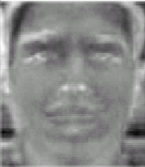
\includegraphics[width=\textwidth]{images/q3_eigenface_ex1.png}
  \end{subfigure}
  \hspace{2em}
  \begin{subfigure}[b]{0.18\textwidth}
    \centering
    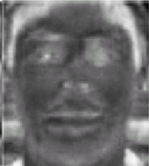
\includegraphics[width=\textwidth]{images/q3_eigenface_ex2.png}
  \end{subfigure}
  \hspace{2em}
  \begin{subfigure}[b]{0.18\textwidth}
    \centering
    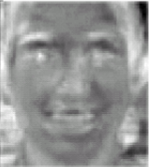
\includegraphics[width=\textwidth]{images/q3_eigenface_ex3.png}
  \end{subfigure}
  \caption{Example of three typical eigenfaces, presented in \cite{lovell_2008}.}
  \label{fig:eigenfaces_ex}
\end{figure}

\newpage
\subsection{Support Vector Machines}

Before describing the methodology, a final section is warranted to introduce the support vector machine (SVM). A SVM is the classifier chosen to perform classification of faces in the testing set using the eigenfaces derived from the training set.

A SVM is a maximum-margin method for linear classification and regression, and substantiates one of the more general class of kernel machines \cite{alpaydin_2020}. A SVM determines an optimal separating hyperplane, which discriminates a set of data points by class such that the distance between the hyperplane and the closest instances of each class is maximised \cite{alpaydin_2020}. The hyperplane refers simply to a decision boundary in the dimensionality of the data; for example, a line in 2D or a plane in 3D \cite{gandhi_2018}. The points closest to the hyperplane on either side are the support vectors, and the minimum distance between these points is the SVM margin \cite{gandhi_2018}. Maximising this margin aims to provide robustness in classifying new data \cite{gandhi_2018}.

The optimal separating hyperplane is defined as a linear combination of the subset of data points which defines the margin \cite{alpaydin_2020}. Consider first the two-class classification problem, where $\mathcal{X} = \{\bm{x}^t, r^t\}$ is the sample, and $r^t=+1$ if $\bm{x}^t\in C_1$ and $r^t=-1$ if $\bm{x}^t\in C_2$ \cite{alpaydin_2020}. That is,
\begin{align}
  \bm{w}^T\bm{x}^t + w_0 \geq +1 \text{ for } r^t = +1 \\
  \bm{w}^T\bm{x}^t + w_0 \geq -1 \text{ for } r^t = -1
\end{align}
where $\bm{w}$ is a vector of weights and $w_0$ is a bias term \cite{alpaydin_2020}. To determine the optimal separating hyperplane, the distance of $\bm{x}^t$ to the discriminant, defined as
\begin{align}
  \frac{r_t(\bm{w}^T \bm{x}^t + w_0)}{||\bm{w}||}
\end{align}
must be maximised \cite{alpaydin_2020}. This may be achieved by minimising $||\bm{w}||$:
\begin{align}
  \min \frac{1}{2} ||\bm{w}||^2 \text{ subject to } r^t(\bm{w}^T\bm{x}^t + w_0) \geq +1, \forall t
\end{align}

Quoting from Alpaydin \cite{alpaydin_2020}, this is a standard quadratic programming problem, and can be solved directly for $\bm{w}$ and $w_0$. This assumes, however, that the classes are linearly separable \cite{alpaydin_2020}. If they are not, then instances may lie insufficiently away from or on the wrong side of the hyperplane \cite{alpaydin_2020}. For these instance, an error is defined based on the deviation from the margin, and is included as a penalty term in the optimisation problem; the SVM then seeks to determine the separating hyperplane incurring the least error \cite{alpaydin_2020}.

The two-class SVM classifier can be extended to a multiclass problem by defining a two-class problem for each class; that is, classifier $g_i(\bm{x})$ determines only whether instances are in class $C_i$, or not \cite{alpaydin_2020}. While it is also possible to construct a single multiclass problem, wherein all hyperplanes are simultaneously optimised, this approach is generally not preferred as the complexity is greater than the decomposition approach for the same outcome \cite{alpaydin_2020}.

In general, the SVM is favourable for a number of reasons, among which include both simplicity and efficiency. A discriminant-based method, the SVM uses Vapnik's principle to avoid solving a more complex problem as an intermediate step than the problem to be solved \cite{alpaydin_2020}. For example, in solving a classification problem it is unnecessary to determine class densities or posterior probabilities where only the boundary between classes need be determined \cite{alpaydin_2020}. The SVM is also memory efficient, in that the optimal hyperplane is in terms of a subset of the original data \cite{alpaydin_2020}. Finally, the popularity of the method means well-founded and reliable implementations are easily available in many machine learning libraries, enabling, in the spirit of Vapnik's principle, the problem of implementing a classifier to be avoided where it is not the aim of an investigation.

\newpage
\section{Methodology}
\subsection{Data Set}

The image data set consists of 33 images of six individuals expressing various facial expressions. On ethical grounds, the individuals are referred to only by number, as individuals 1 through 6. The training set of images consists of one image of each individual, as presented in Figure \ref{fig:training_imgs}. All images are 3-channel greyscale and $128\times128$ pixels.

\begin{figure}[ht]
  \centering
  \begin{subfigure}[b]{0.15\textwidth}
    \centering
    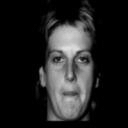
\includegraphics[width=\textwidth]{images/q3_face_1a.png}
  \end{subfigure}
  \hfill
  \begin{subfigure}[b]{0.15\textwidth}
    \centering
    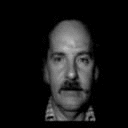
\includegraphics[width=\textwidth]{images/q3_face_2a.png}
  \end{subfigure}
  \hfill
  \begin{subfigure}[b]{0.15\textwidth}
    \centering
    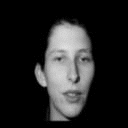
\includegraphics[width=\textwidth]{images/q3_face_3a.png}
  \end{subfigure}
  \hfill
  \begin{subfigure}[b]{0.15\textwidth}
    \centering
    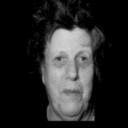
\includegraphics[width=\textwidth]{images/q3_face_4a.png}
  \end{subfigure}
  \hfill
  \begin{subfigure}[b]{0.15\textwidth}
    \centering
    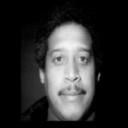
\includegraphics[width=\textwidth]{images/q3_face_5a.png}
  \end{subfigure}
  \hfill
  \begin{subfigure}[b]{0.15\textwidth}
    \centering
    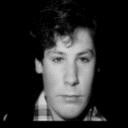
\includegraphics[width=\textwidth]{images/q3_face_6a.png}
  \end{subfigure}
  \caption{Training set consisting of one face each of individuals 1 to 6 (from left to right).}
  \label{fig:training_imgs}
\end{figure}

Approaching the problem as a typical machine learning model evaluation, the testing set should consist only of the remaining 27 images, representing unseen data on which the ability of the model to generalise is tested. However, for this investigation, all 33 images are considered in determining the accuracy of the model.

\subsection{Eigenface Method}

This section describes the implementation of the eigenface method. As part of the method, two implementations of PCA are provided in the source code of Appendix \ref{app:face_recognition_py}: the scikit-learn implementation, and a manual implementation. Indeed, the methods are fundamentally identical, both \cite{sklearn_2023} applying the singular value decomposition suggested by Lovell and Chen \cite{lovell_2008}. Practically, the scikit-learn implementation is, of course, more robust; yet, a manual implementation is included in response to the apparent necessity of the author proving an ability to program a simple and widely published algorithm where well-founded implementations already exist.

In this section, PCA is implemented using the scikit-learn library, which exposes an optimised and user-friendly implementation of the PCA method \cite{sklearn_2023}. The manual implementation may be referred to in Appendix \ref{app:face_recognition_py}, though the author assures that the outcomes are, naturally, identical. An SVM classifier, also from the scikit-learn API \cite{sklearn_2023b}, is trained on the six training images after being transformed by the eigenfaces. In detail:

\begin{enumerate}
  \item The 33 images are loaded, and a training set is defined as a subset of the entire set.

  \item The images are converted from 3-channel greyscale to single-channel greyscale.

  \item The images are flattened into a single vector each, and the training and testing images are separately stacked into two matrices of dimensions $6\times16,384$ and $33\times16,384$, respectively.

  \item The image vectors are labelled according to the enumeration presented in Figure \ref{fig:training_imgs}.

  \item A PCA model is defined and fitted to the training images using the scikit-learn library:
  \begin{center}
    \texttt{pca = sklearn.decomposition.PCA().fit(X\_train)}
  \end{center}
  where \texttt{X\_train} is the matrix of training image vectors. As an aside, the attribute:
  \begin{center}
    \texttt{pca.components\_[0...5]}
  \end{center}
  now contains the principal components (eigenfaces) derived from the training set. Each can be reshaped from a vector back into the original dimensions and viewed as an image.

  \item The eigenfaces can now be used to transform the training and testing images, in preparation for classification:
  \begin{center}
    \texttt{X\_train\_pca = pca.transform(X\_train)}
  \end{center}
  and similarly for the larger matrix of test images, \texttt{X\_test} $\mapsto$ \texttt{X\_test\_pca}.

  \item Finally, a SVM classifier can be defined and fitted to the training data using scikit-learn:
  \begin{center}
    \texttt{svm = sklearn.svm.SVC().fit(X\_train\_pca, y\_train)}
  \end{center}
  where the vector \texttt{y\_train} contains the labels of the training images.

  \item The result can be observed using the \texttt{classification\_report} from scikit-learn:
  \begin{center}
    \texttt{sklearn.metrics.classification\_report(y\_test, svm.predict(X\_test\_pca))}
  \end{center}
  where the vector \texttt{y\_test} contains the labels of the testing images.

\end{enumerate}

In the final step, the SVM predicts labels for each of the eigenface-transformed image vectors in the matrix \texttt{X\_test\_pca}, and compares these to \texttt{y\_test} to determine the model accuracy.

The classification report is presented:

\vspace{1em}
\begin{lstlisting}[numbers=none, xleftmargin=5em]
              precision    recall  f1-score   support

           0       1.00      1.00      1.00         7
           1       1.00      1.00      1.00         4
           2       1.00      0.90      0.95        10
           3       1.00      1.00      1.00         4
           4       0.80      1.00      0.89         4
           5       1.00      1.00      1.00         4

    accuracy                           0.97        33
   macro avg       0.97      0.98      0.97        33
weighted avg       0.98      0.97      0.97        33
\end{lstlisting}

From the above report, the model evidently achieves 97\% classification accuracy. One image of individual 3 (labelled 2 due to zero-indexing) is misclassified as individual 5 (labelled 4). It is, however, not evident which image is misclassified.

\subsection{Simple GUI}

To assist in validating the classification results, and determining in which cases misclassifications occur, a simple web-based GUI is developed in conjunction with the eigenface implementation. The framework of choice is Gradio \cite{gradio_2023}, and courtesy of Gradio's API, this is very simple:

\begin{enumerate}
  \item The GUI interface is defined as accepting an image and producing an image as output:
  \begin{center}
    \texttt{app = gr.Interface(fn=face\_classifier, inputs="image", outputs="image")}
  \end{center}

  \item The function \texttt{face\_classifier} is defined to wrap the eigenface implementation, such that an input image is prepared, transformed and classified by the trained PCA and SVM.

  \item The GUI is launched using:
  \begin{center}
    \texttt{app.launch()}
  \end{center}

\end{enumerate}
\vspace{1em}

This launches a local server running the GUI, which can be accessed in the browser at the default URL: http://127.0.0.1:7860/. The appearance of the GUI and an example user flow is presented in the following section.

\newpage
\section{Results}

The trained SVM classifier achieves a 97\% accuracy on the testing images, representing 32 out of 33 faces correctly recognised. The sole misidentification is presented in Figure \ref{fig:misidentification}.

\begin{figure}[ht]
  \centering
  \begin{subfigure}[b]{0.2\textwidth}
    \centering
    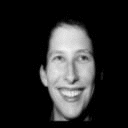
\includegraphics[width=\textwidth]{images/q3_face_3c.png}
    \caption{Face 3c}
  \end{subfigure}
  \hspace{3em}
  \begin{subfigure}[b]{0.2\textwidth}
    \centering
    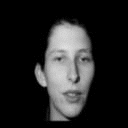
\includegraphics[width=\textwidth]{images/q3_face_3a.png}
    \caption{Face 3a}
  \end{subfigure}
  \hspace{3em}
  \begin{subfigure}[b]{0.2\textwidth}
    \centering
    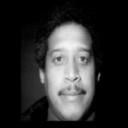
\includegraphics[width=\textwidth]{images/q3_face_5a.png}
    \caption{Face 5a}
  \end{subfigure}
  \caption{Face 3c is misidentified as individual 5; training faces of individuals 3 and 5 shown.}
  \label{fig:misidentification}
\end{figure}

As an extension to the solution, a simple web-based GUI built using Gradio \cite{gradio_2023} was developed. The GUI enables the user to select an image from the testing set in the left pane, and the recognised face from the training set is displayed in the right pane. The output can be flagged to log the input and output to a file. Figure \ref{fig:gui} demonstrates the use of the GUI.

\begin{figure}[ht]
  \centering
  \begin{subfigure}[b]{0.95\textwidth}
    \centering
    
\includegraphics[width=\textwidth]{images/q3_gui_1.png}
    \caption{Landing screen}
  \end{subfigure}
  \\[1em]
  \begin{subfigure}[b]{0.95\textwidth}
    \centering
    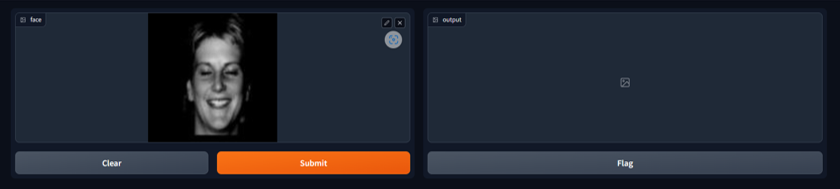
\includegraphics[width=\textwidth]{images/q3_gui_2.png}
    \caption{Image selected from testing set}
  \end{subfigure}
  \\[1em]
  \begin{subfigure}[b]{0.95\textwidth}
    \centering
    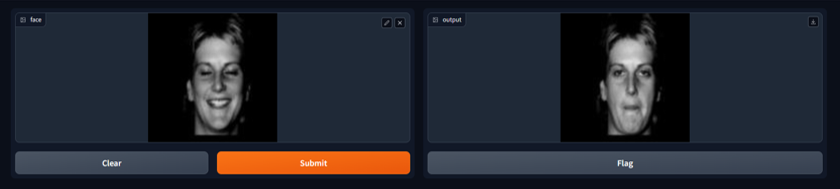
\includegraphics[width=\textwidth]{images/q3_gui_3.png}
    \caption{Recognised face produced from training set}
  \end{subfigure}
  \caption{A simple GUI built with Gradio, enabling a user to validate recognition results.}
  \label{fig:gui}
\end{figure}

\newpage
\section{Discussion}

This report has presented an implementation of the eigenface method for recognition of faces. The implementation is applied to a small data set of 33 images of the faces of six individuals. Of these, one image of each individual, six images in total, is used to generate the eigenfaces and train the SVM classifier. The classifier is then tested against all 33 images, producing a 97\% accuracy rate. This represents 32 out of the 33 images correctly recognised, with the single misidentification having been presented in the previous section.

In understanding the reason for the misidentification, the first step is to understand the eigenface representation of the misidentified face. An image transformed by a set of eigenfaces is represented as a weighted sum of the eigenfaces. Given six eigenfaces, as in this case, the image vector transformed by the eigenfaces yields a 6-vector of corresponding weights. The following table compares the misidentified face with the correct and incorrectly recognised training faces:

\begin{table}[ht]
  \small \centering \restretch{1.2}
  \begin{tabularx}{0.78\textwidth}{l r r r r r r}
    \toprule
    \textbf{Face}     & $\bm{u}_1$ & $\bm{u}_2$ & $\bm{u}_3$ & $\bm{u}_4$ & $\bm{u}_5$ & $\bm{u}_6$ \\
    \midrule
    3c: misidentified &   -1101.71 &   -1367.71 &     134.83 &      30.57 &    -160.32 &      11.81 \\
    3a: correct       &    -484.35 &   -1180.57 &    1733.97 &     896.03 &     -98.61 &       2.37 \\
    5a: incorrect     &   -1790.09 &   -1743.83 &    -367.29 &   -1251.14 &    -703.20 &      -0.70 \\
    \bottomrule
  \end{tabularx}
\end{table}

The column $\bm{u}_i$ lists the weights associated with eigenface $i$ for the particular image. In the representation of the first three eigenfaces, which explain the majority of variance, the misidentified face is clearly more similar to individual 5 as compared to individual 3.

This can be further verified by visually observing the first three eigenfaces, as in Figure \ref{fig:eigenfaces_res}.

\begin{figure}[ht]
  \centering
  \begin{subfigure}[b]{0.2\textwidth}
    \centering
    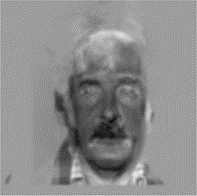
\includegraphics[width=\textwidth]{images/q3_eigenface_res1.png}
  \end{subfigure}
  \hspace{2em}
  \begin{subfigure}[b]{0.2\textwidth}
    \centering
    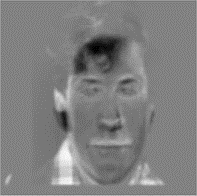
\includegraphics[width=\textwidth]{images/q3_eigenface_res2.png}
  \end{subfigure}
  \hspace{2em}
  \begin{subfigure}[b]{0.2\textwidth}
    \centering
    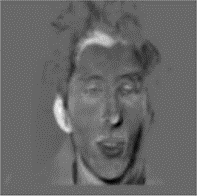
\includegraphics[width=\textwidth]{images/q3_eigenface_res3.png}
  \end{subfigure}
  \caption{First three eigenfaces derived from training images.}
  \label{fig:eigenfaces_res}
\end{figure}

From the above, alongside the original images of faces 3c, 3a and 5a, pictured in Figure \ref{fig:misidentification}, an intuition can be developed surrounding the cause of the misidentification. Consider the face shape and shadowing in the first and third eigenfaces; image 3c is more similar to 5a than 3a in both regards. Consider also the ear position, highlighted in the third eigenface; 3c is again more similar to 5a. Finally, and though not immediately evident from the eigenfaces, it is presumed possible that the wide smile of individual 3 in image 3c generates a better match with the moustasche of individual 5 than the narrow mouth position in image 3a. These characteristics, no doubt alongside other less obvious features, contribute to the misidentification of image 3c.

More generally, the limitations of the eigenface method in robustness against variations in facial expression and lighting are well documented \cite{lovell_2008}. While improvements such as ACPA have been demonstrated to offer a marked improvement in robustness \cite{lovell_2008}, the method does not achieve a competitive standard of accuracy compared to modern deep learning techniques \cite{benito_2017}. As such, eigenfaces have for some time been superseded by modern approaches \cite{elec4630_2023}.

\newpage
\section{Conclusion}

In summary, this report presents a largely successful implementation of the eigenface method for face recognition. The implementation achieves a 97\% accuracy rate on a small data set of 33 images. With dimensionality reduction being core to its approach, the eigenface method represents an efficient solution to facial recognition, because many features in images are highly correlated. Nevertheless, the simplicity of the method results in inherent robustness limitations, and eigenfaces have been superseded for face recognition by modern deep learning techniques.
